\documentclass[conference,a4paper]{IEEEtran}

\IEEEoverridecommandlockouts
\usepackage[utf8]{inputenc}
\usepackage[T1]{fontenc}
\usepackage[brazilian]{babel}
\usepackage{amsmath,amssymb}
\usepackage{graphicx}
\usepackage{url}

\begin{document}

\title{Heurística para alocação de produtos em armazém\\
com capacidade e frequência de demanda}

\author{\IEEEauthorblockN{Rafael Andrade Mirapalheta}
\IEEEauthorblockA{Universidade Federal do Rio Grande do Norte\\
Natal, Brasil}}

\maketitle

\begin{abstract}
A alocação de produtos a posições de armazenagem, com custo de acesso e custo de separação por coocorrência, é formulada como um problema de atribuição com termo quadrático e restrição de capacidade.
O algoritmo do trabalho é uma busca local por troca de posições, partida de um guloso por frequência, com o custo de cada troca calculado de forma incremental.
Nas instâncias geradas de 20 a 200 produtos, o custo total cai de cerca de 21\% a 39\% em relação ao guloso.
O valor coincide com o da mesma busca avaliando a função inteira.
Na instância de 200 produtos, o tempo foi de 2,3~s, contra 117~s do recálculo completo.
\end{abstract}

\begin{IEEEkeywords}
alocação em armazém, heurística construtiva, busca local, atribuição quadrática
\end{IEEEkeywords}

\section{Introdução}
A posição de um produto no armazém altera o percurso de quem o separa.
Itens de alta frequência convêm posições de acesso barato.
Itens que saem no mesmo pedido convêm posições próximas.
Este trabalho apresenta uma heurística para esse compromisso, sob limite de capacidade de cada posição.
A construção inicial ordena os produtos pela frequência.
A busca troca posições enquanto o custo total diminui.
O cálculo incremental evita recompor a função objetivo a cada candidato.

\section{Descrição do problema}
Há \(n\) produtos e \(m\) posições, com \(m \ge n\).
O produto \(i\) tem volume \(v_i\) e frequência de acesso \(d_i\).
A posição \(j\) tem capacidade \(C_j\) e custo de acesso \(c_j\).
\(D_{pq}\) é a distância entre as posições \(p\) e \(q\).
\(q_{ik}\) é o número de pedidos em que os produtos \(i\) e \(k\) aparecem juntos.
A variável \(x_{ij} \in \{0,1\}\) vale 1 quando o produto \(i\) ocupa a posição \(j\).
Cada produto ocupa uma única posição, e cada posição recebe no máximo um produto.

O custo de acesso e o custo de separação são
\begin{align}
C_{\mathrm{acesso}} &= \sum_{i=1}^{n} \sum_{j=1}^{m} d_i \, c_j \, x_{ij}, \\
C_{\mathrm{sep}} &= \sum_{1 \le i < k \le n} q_{ik} \sum_{p=1}^{m} \sum_{r=1}^{m} D_{pr} \, x_{ip} \, x_{kr}.
\end{align}
Com pesos \(\alpha \ge 0\) e \(\beta \ge 0\), o objetivo é
\begin{equation}
\min \; \alpha \, C_{\mathrm{acesso}} + \beta \, C_{\mathrm{sep}}
\end{equation}
sujeito a
\begin{align}
\sum_{j=1}^{m} x_{ij} &= 1 && \forall i, \\
\sum_{i=1}^{n} x_{ij} &\le 1 && \forall j, \\
v_i \, x_{ij} &\le C_j && \forall i,j, \\
x_{ij} &\in \{0,1\}.
\end{align}

\section{Complexidade}
Sem o termo de separação, as restrições descrevem uma atribuição com custos lineares.
O produto \(q_{ik} D_{pr} x_{ip} x_{kr}\) torna a escolha das posições combinatória.
O método deste trabalho é uma heurística e não traz fator de aproximação.

\section{Heurísticas já apresentadas}
Kim, Méndez e Jimenez decidem a posição de um item frequente e a ordem que agrupa itens pedidos juntos \cite{kim2020}.
Wutthisirisart, Noble e Chang separam o procedimento em duas fases: ordenam pela relação com os pedidos e depois alocam \cite{wutthisirisart2015}.
Chou, Yu e Wu medem o ganho de trocar dois itens de posição quando a correlação entra no custo \cite{chou2023}.

\section{Instâncias}
Não há um banco público consolidado para esta variante com volume, capacidade e coocorrência.
As instâncias do trabalho são pastas de texto, com campos separados por \texttt{;} ou \texttt{,}:
\begin{itemize}
\item \texttt{produtos.txt}: identificador, nome, volume, frequência;
\item \texttt{posicoes.txt}: identificador, capacidade, custo de acesso;
\item \texttt{distancias.txt}: origem, destino, distância;
\item \texttt{coocorrencia.txt}: produto, produto, vezes no mesmo pedido;
\item \texttt{pesos.txt}: \(\alpha\) e \(\beta\).
\end{itemize}
O núcleo quadrático do problema aparece no QAPLIB\footnote{\url{https://www.opt.math.tugraz.at/qaplib/}}.
Essas instâncias não trazem volume, capacidade nem custo de acesso, e por isso não servem de referência numérica para a função deste trabalho.

As instâncias do experimento saem de \texttt{tools/gerar\_instancias.cpp}.
Cada arquivo é sorteado com semente 21, por um gerador congruente linear.
Os tamanhos são 20, 50, 100 e 200 produtos.
O número de posições é \(m = n + \lfloor n/5 \rfloor\).
O volume de cada produto é inteiro de 2 a 12 e a frequência é inteira de 1 a 180.
A capacidade da posição \(j\) é \(20 + (j \bmod 5)\), sempre maior que qualquer volume, então a restrição de capacidade não elimina alocações nesses arquivos.
O custo de acesso da posição \(j\) é \(1 + \lfloor (j-1)/2 \rfloor\).
A distância entre duas posições é o módulo da diferença dos identificadores.
A coocorrência liga cada produto \(i\) a \(i+1\), \(i+3\), \(i+7\) e \(i+12\), quando o outro identificador existe, com contagem inteira de 2 a 40.
Os pesos são \(\alpha = \beta = 1\).
A pasta \texttt{data/armazem}, com 4 produtos e 5 posições, permanece como caso curto em que a capacidade de fato impede algumas alocações.

\section{Implementação}
O programa está em C++17 e usa apenas a biblioteca padrão.
O algoritmo do trabalho é a heurística de custo incremental.
O guloso só constrói a solução inicial.
A busca com recálculo completo percorre a mesma vizinhança e serve para conferir o custo.

\subsection{Guloso por frequência}
Ordena os produtos por \(d_i\) decrescente e as posições por \(c_j\) crescente.
Cada produto recebe a primeira posição livre cuja capacidade comporta \(v_i\).
A ordenação usa a frequência, não a razão entre demanda e espaço do índice cubo por pedido.

\subsection{Busca local}
A partir da solução gulosa, cada passagem examina os pares de produtos já posicionados.
A troca só é aceita se as duas posições comportam os volumes.
Aplica-se a troca de maior redução do custo total.
O laço para quando nenhuma troca melhora o custo.
Na versão de conferência, cada candidato recalcula \(C_{\mathrm{acesso}}\) e \(C_{\mathrm{sep}}\) por inteiro.

\subsection{Heurística com custo incremental}
A vizinhança e o critério de parada são os da busca local.
Para os produtos \(a\) e \(b\) nas posições \(p\) e \(r\), a variação de acesso é
\begin{equation}
(d_a - d_b)\,(c_r - c_p).
\end{equation}
A variação de separação soma, para cada outro produto \(o\) na posição \(s\),
\begin{equation}
q_{ao}(D_{rs} - D_{ps}) + q_{bo}(D_{ps} - D_{rs}).
\end{equation}
O delta da troca é \(\alpha\) vezes a primeira variação mais \(\beta\) vezes a segunda.
Só entram os pares ligados a \(a\) ou a \(b\).

\subsection{Execução}
Na pasta \texttt{PAA-T01}, sem biblioteca extra.
Pelo compilador, direto:
\begin{verbatim}
c++ -std=c++17 -O2 -I lib -o paa_t01 \
  source/main.cpp source/program.cpp \
  lib/instance.cpp lib/cost.cpp \
  lib/greedy.cpp lib/local_search.cpp \
  lib/improved.cpp
c++ -std=c++17 -O2 -o gerar_instancias \
  tools/gerar_instancias.cpp
./gerar_instancias
./paa_t01
\end{verbatim}
Pelo CMake, a configuração padrão é Release:
\begin{verbatim}
cmake -S . -B build
cmake --build build
./build/gerar_instancias
./build/source/paa_t01
\end{verbatim}
No menu, a opção 1 lista as pastas de \texttt{data/} e carrega pelo número.
A opção 4 executa a heurística.
As opções 2 e 3 executam o guloso e a busca com recálculo completo.
Ao fim, a tela mostra o posicionamento, o custo e o tempo, e o programa grava \texttt{resultados/<instância>/relatorio-heuristica.txt} e \texttt{melhor-solucao-heuristica.txt}.
A opção 6 mostra \texttt{resultados/log.txt}.

\section{Análise do algoritmo}
A ordenação do guloso custa \(O(n \log n + m \log m)\).
A varredura das posições livres, no pior caso, custa \(O(nm)\).
Na busca local, cada passagem examina \(O(n^2)\) pares.
Recalcular o custo de um par custa \(O(n^2)\), logo a passagem custa \(O(n^4)\).
No cálculo incremental, cada par custa \(O(n)\), e a passagem custa \(O(n^3)\).
O número de passagens depende da instância: cada uma reduz o custo, e o laço termina num ótimo local da vizinhança de trocas.

\section{Resultados}
As quatro instâncias geradas foram resolvidas uma vez, com o programa compilado em \texttt{-O2}.
Todas as alocações posicionaram todos os produtos e respeitaram a capacidade.
A ocupação das posições usadas ficou entre 30\% e 32\%: a capacidade gerada comporta qualquer produto e o volume médio é menor.
A busca com recálculo completo e a heurística incremental produziram o mesmo custo em todas as instâncias.
A Tabela~\ref{tab:custos} compara o guloso com essa solução.
A Tabela~\ref{tab:tempos} compara os tempos das duas avaliações da mesma vizinhança.
A Figura~\ref{fig:custo} e a Figura~\ref{fig:tempo} mostram as mesmas execuções.

\begin{table*}[t]
\caption{Custo do guloso e da heurística incremental.
A busca com recálculo completo atingiu os mesmos valores da heurística.}
\label{tab:custos}
\centering
\scriptsize
\begin{tabular}{|l|r|r|r|r|r|r|}
\hline
Instância & Acesso G & Sep.\ G & Total G & Acesso H & Sep.\ H & Total H \\
\hline
n20  & 5\,204 & 8\,513 & 13\,717 & 5\,990 & 4\,896 & 10\,886 \\
n50  & 35\,212 & 56\,410 & 91\,622 & 45\,908 & 18\,584 & 64\,492 \\
n100 & 136\,820 & 268\,536 & 405\,356 & 192\,424 & 61\,475 & 253\,899 \\
n200 & 567\,460 & 1\,124\,843 & 1\,692\,303 & 793\,994 & 231\,939 & 1\,025\,933 \\
\hline
\end{tabular}
\end{table*}

\begin{table}[htbp]
\caption{Uma execução.
Trocas aceitas até o ótimo local e tempo das duas avaliações.}
\label{tab:tempos}
\centering
\scriptsize
\begin{tabular}{|l|r|r|r|}
\hline
Instância & Trocas & Busca local & Heurística \\
\hline
n20  & 18  & 0,5~ms & 0,1~ms \\
n50  & 70  & 90~ms  & 5,6~ms \\
n100 & 188 & 3,8~s  & 116~ms \\
n200 & 353 & 117~s  & 2,3~s \\
\hline
\end{tabular}
\end{table}

\begin{figure}[htbp]
\centering
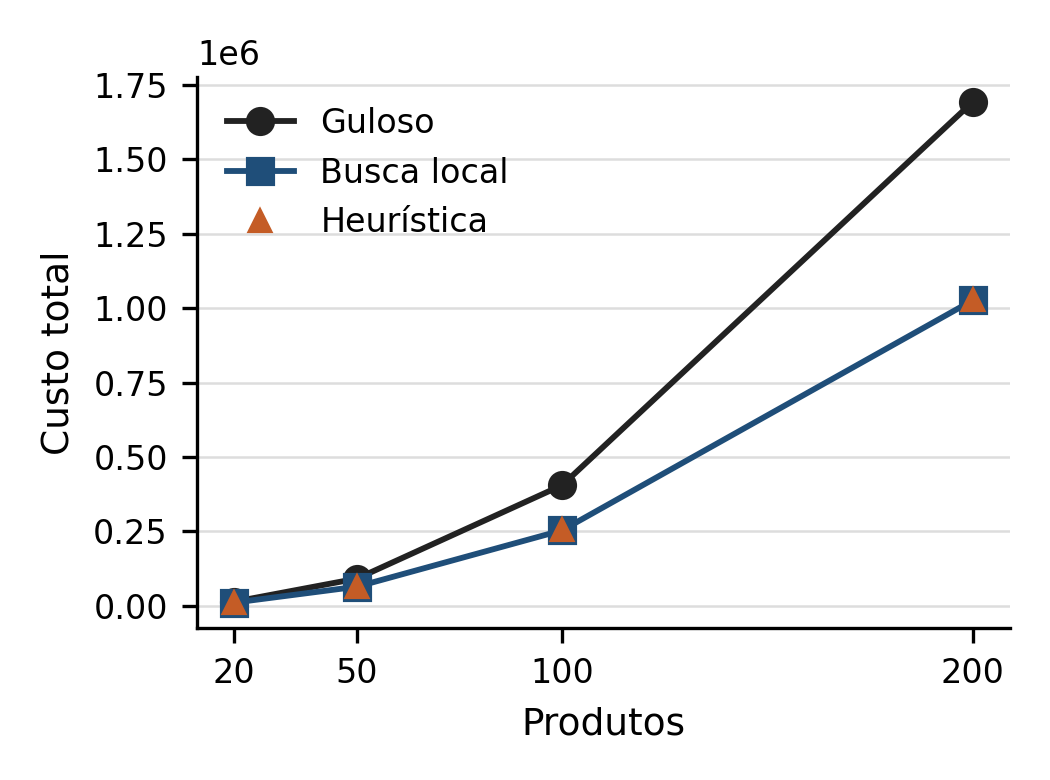
\includegraphics[width=\columnwidth]{custo-total.png}
\caption{Custo total nas instâncias geradas.
A busca local e a heurística coincidem.}
\label{fig:custo}
\end{figure}

\begin{figure}[htbp]
\centering
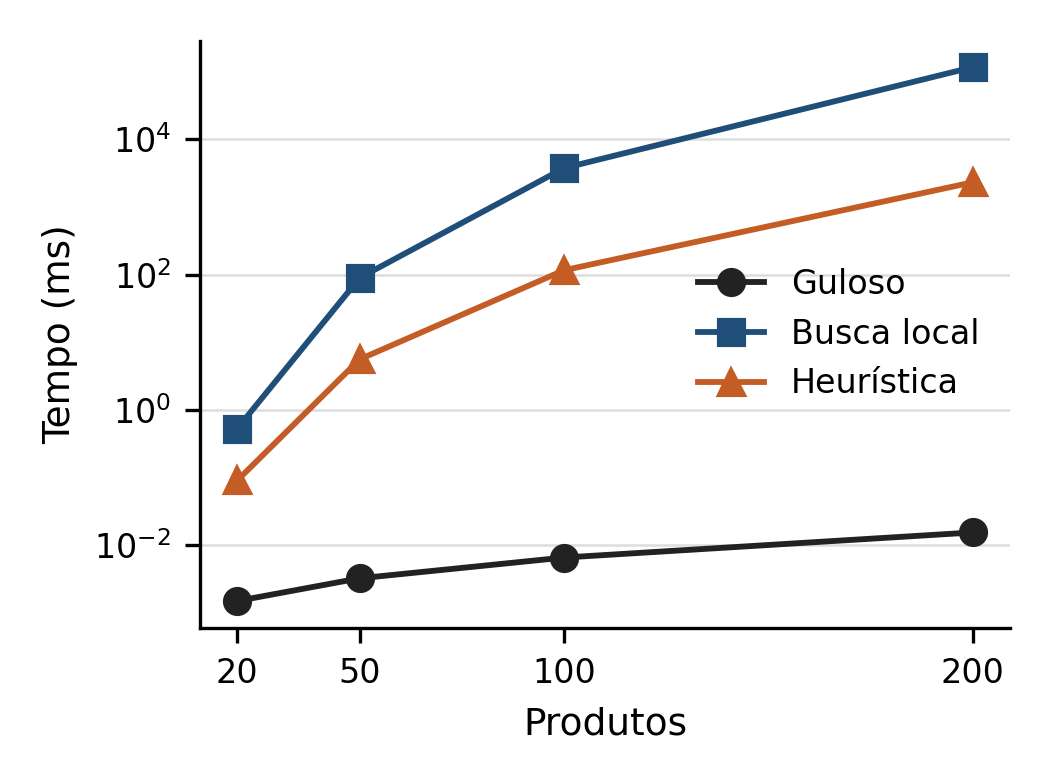
\includegraphics[width=\columnwidth]{tempo.png}
\caption{Tempo de uma execução.
O eixo vertical está em escala logarítmica.}
\label{fig:tempo}
\end{figure}

O guloso coloca a frequência nas posições baratas e deixa a coocorrência de lado.
A busca aceita pagar mais acesso para reduzir a separação, e o total cai: cerca de 21\% em n20, 30\% em n50, 37\% em n100 e 39\% em n200.
Em n200, a separação cai de 1\,124\,843 para 231\,939 e o acesso sobe de 567\,460 para 793\,994.
O tempo do guloso ficou abaixo de 1~ms nas quatro instâncias.
Na n200, a avaliação incremental foi cerca de 50 vezes mais rápida que o recálculo completo, com o mesmo ótimo local e as mesmas 353 trocas.

Não há número publicado para estas instâncias.
Os ótimos do QAPLIB não se aplicam: falta o custo linear de acesso, e as matrizes de fluxo e distância não são as de lá.
A referência interna é o guloso por frequência e a mesma busca local com avaliação completa.

\section{Conclusão}
A heurística incremental, partida do guloso por frequência, reduz o custo total nas instâncias geradas de 20 a 200 produtos.
A redução vem da separação dos itens que coocorrem, e supera o aumento do custo de acesso.
O custo obtido é o mesmo da busca que recalcula a função inteira, com passagem \(O(n^3)\) em vez de \(O(n^4)\).
O limite observado é o ótimo local da vizinhança de trocas.

\begin{thebibliography}{9}
\bibitem{kim2020}
J.~Kim, F.~Méndez, and J.~Jimenez, ``Storage location assignment heuristics based on slot selection and frequent itemset grouping for large distribution centers,'' \emph{IEEE Access}, vol.~8, pp.~189025--189035, 2020.

\bibitem{wutthisirisart2015}
P.~Wutthisirisart, J.~S. Noble, and C.~A. Chang, ``A two-phased heuristic for relation-based item location,'' \emph{Computers \& Industrial Engineering}, vol.~82, pp.~94--102, 2015.

\bibitem{chou2023}
Y.-L. Chou, V.~F. Yu, and C.-H. Wu, ``An efficient data-driven method for storage location assignment under item correlation considerations,'' \emph{International Journal of Systems Science: Operations \& Logistics}, vol.~10, no.~1, Art.~no.~2228447, 2023.
\end{thebibliography}

\end{document}
